% -*- coding: utf-8 -*-
%%%%%%%%%%%%%%%%%%%%%%%%%%%%%%%%%%%%%%%%%%%%%%%%
%%%%%%%%%%%%%%%%%%%%%%%%%%%%%%%%%%%%%%%%%%%%%%%%
%%%%%%%%%%%%%%%%%%%%%%%%%%%%%%%%%%%%%%%%%%%%%%%%
\chapter{ヒューリスティック探索 (Heuristic Search)}
\label{ch:heuristic-search}

\ref{ch:blind-search}章では問題の知識を利用しないグラフ探索手法について解説した。
本章では問題の知識を利用することでより効率的なグラフ探索を行う手法、特にヒューリスティック探索について解説する。

\section{ヒューリスティックとは?}
\label{sec:heursitic}

経路探索問題を幅優先探索で解くことを考えよう。
図\ref{fig:grid}の初期状態からゴールへの最短経路の長さは18である。このとき、幅優先探索は図\ref{fig:grid-brfs}の領域を探索する。
しかし人間が経路探索を行うときにこんなに広い領域を探索しないだろう。グリッドの右側、ゴールのある方向に向かってのみ探索するだろう。なぜか。
それは人間が問題の特徴を利用して、このノードを探索したほうがよいだろう、という推論を働かせているからである。
問題の特徴を利用してノードの{\bf 有望さ}を\define{ヒューリスティック関数}{heuristic function}{ヒューリスティックかんすう}として定量化し、ヒューリスティック関数を利用した探索アルゴリズムをヒューリスティック探索と呼ぶ。
ヒューリスティック関数は人間が自分の知識を利用してコーディングする場合と、自動的にヒューリスティックを生成する場合もある。

\begin{figure}
\centering
\subfloat[幅優先探索]{
\includegraphics[width=0.45\textwidth]{figures/grid-brfs.png}
\label{fig:grid-dijkstra}
} \hspace{4pt}
\subfloat[ヒューリスティック探索]{
\includegraphics[width=0.45\textwidth]{figures/grid-astar-mdheuristic.png}
\label{fig:grid-astar-mdheuristic}
}
\end{figure}


%\captionlistentry[todo]{ヒューリスティックとは: grid, grid-brfsの図を挿入}
%{\TODO ヒューリスティックとは: grid, grid-brfsの図を挿入}

\section{ヒューリスティック関数 (Heuristic Function)}
\label{sec:heuristic-function}
ヒューリスティック関数は状態の有望さの評価値であり、多くの場合その状態からゴールまでの最短距離の見積もりであることが多い \cite{hart68formal}。

\ddef{ヒューリスティック関数、heuristic function}{
	ヒューリスティック関数$h$はノードの評価関数である。$h: V \rightarrow \mathbb{R}_{\geq 0}$
}
ヒューリスティックの値が小さいノードほどゴールに近いと推測できるので、探索ではヒューリスティック値が小さいノードを優先して展開する。
ヒューリスティック関数の値をそのノードの$h$値と呼ぶ。

ヒューリスティック関数の望ましい性質として、まず正確である方が望ましい。すなわち、$h$値が実際のゴールまでの最短距離に近いほど、有用な情報であると言える。
ノード$n$からゴールまでの正しい最短コストを$h^*$とする。
ヒューリスティック関数$h$が任意の$n$に対して$h(n) = h^*(n)$である場合、\define{完璧なヒューリスティック}{Perfect Heuristic}{かんぺきなヒューリスティック}と呼ぶ。完璧なヒューリスティックがある場合、ほとんどの場合その問題を一瞬で解くことができる。現実には完璧なヒューリスティックはなかなか得られないが、ヒューリスティック関数がこれに近いほど必要な展開ノード数が小さいことが多い\cite{helmert:08}。
%完璧なヒューリスティック関数がある場合、A*探索は
反対に役に立たないヒューリスティック関数は$h(n) = 0$などの定数関数である。これはどのノードに対してもゴールまでの距離が同じだと推測しているということであり、つまり何も主張をしていない。このようなヒューリスティックをブラインドヒューリスティックと呼ばれる。ブラインドヒューリスティックを使った探索は、\ref{ch:blind-search}章で扱った情報なし探索の一種といえる。


もう一つ望ましい性質は$h$値が最適解コストの下界である場合である。
\ref{sec:astar-search}章で解説するが、$h$値が最短距離の下界である場合、それを用いた効率的な探索アルゴリズム(A*探索、重み付きA*探索)において解コストに理論的保証が得られることが広く知られている。
$h$値が常に最適解コストの下界であるヒューリスティック関数を許容的なヒューリスティックと呼ぶ。

\ddef{許容的なヒューリスティック、admissible heuristic}{
	ヒューリスティック関数$h$は最適解のコストの下界である場合、許容的である。すなわち、全てのノード$u \in V$に対して$h(u) \leq h^*(u)$が成り立つ。
}

ただし、$h^*(u)$はノード$u$からゴールノード集合$T$のいずれかへたどり着くための最短経路である。%$h^*$はパーフェクトヒューリスティックと呼ぶ。

一般に、許容的なヒューリスティックを得る方法としては、元問題の{\bf 緩和問題}を解き、その最適解コストをヒューリスティック値とすることである。ある問題の緩和問題とは、解集合に元の問題の解を含む問題を指す。要するに元の問題より簡単な問題である\footnote{解が多いほど簡単であるとは一概には言えないが}。

%許容的よりも強い性質としてとして無矛盾性がある。

もう一つ重要な性質は無矛盾性である。

\ddef{無矛盾なヒューリスティック、consistent heuristic}{
	ヒューリスティック関数$h$は全てのノードのペア$(u, v)$に対して
        \begin{equation}
                h(u) \leq h(v) + k(u,v)
        \end{equation}
        が成り立つ場合、無矛盾である。$k(u, v)$は$u$から$v$への最小コストである (経路がない場合$k = \infty$とする)。
}

無矛盾性は特に\ref{sec:astar-search}章で後述するA*探索において探索の効率性に重要な性質である。
また、無矛盾なヒューリスティックのうちゴールノードの$h$値が0となるヒューリスティックは許容的である。

\dtheorem{
ゴールノード$n \in T$に対して$h(n) = 0$となる無矛盾なヒューリスティックは許容的なヒューリスティックである。
}

\begin{proof}
        すべての状態$u \in S$に対して以下が成り立つ。
\begin{align}
	h(u) &\leq h(n) + k(u, n) \\
             &= k(u, n) \\
             &= h^*(u)
\end{align}
        よって$h(s) \leq h^*(n)$より許容的である。
% あるノード$n_0$からゴールノード$n_k \in T$への最短経路(ノードの列)を$(n_0, n_1,...)$と置く。無矛盾なヒューリスティック$h(n)$は
% \begin{align}
% 	h(n_0) &\leq h(n_1) + w(n_0, n_1) \\
% 			&\leq h(n_2) + w(n_0, n_1) + w(n_1, n_2) \\
% 			&... \\
% 			&\leq h(n_k) + \sum_{i=0..k-1}(w(n_i,n_{i+1})) \\
% 			&= h^*(n_0)
% \end{align}
% よって$h(n_0) \leq h^*(n_0)$より許容的である。

\end{proof}

ゴールノードに対してヒューリスティック値が$0$になるヒューリスティック関数を作ることは簡単である。
ヒューリスティックの無矛盾性は証明することは難しそうであるが、実はシンプルな導き方がある。そのためにまず単調性を定義する。

\ddef{単調なヒューリスティック、monotone heuristic}{
	ヒューリスティック関数$h$は全てのエッジ$e = (u, v) \in E$に対して$h(u) \leq h(v) + w(u,v)$が成り立つ場合、無矛盾である。
}

単調なヒューリスティックは無矛盾性の定義と比較して、ノードのペア$(u, v)$が直接繋がっているという制約がある分、弱い性質に思えるかもしれない。しかし実は単調性と無矛盾性は同値である。


\dtheorem{
        単調性と無矛盾性は同値である。
}
\dproof{
        無矛盾性であるならば単調性であることは自明である。
        単調性が成り立つ場合に無矛盾であることを示す。
        $(u, v)$に経路がない場合$k=\infty$なので
\begin{align}
	h(n_0) &\leq h(n_1) + w(n_0, n_1) \\
			&\leq h(n_2) + w(n_0, n_1) + w(n_1, n_2) \\
			&... \\
			&\leq h(n_k) + \sum_{i=0..k-1}(w(n_i,n_{i+1})) \\
\end{align}
        $u = n_0, v = n_k$とすると無矛盾性が成り立つ。

}

よって、無矛盾性を示すために必要なのは直接つながっているノードのペアに対して$h(u) \leq h(v) + w(u,v)$が成り立つことを示せばよい。これを示すことは比較的にシンプルである。

後述するA*探索においてこれらのアルゴリズムの性質は非常に有用である。
%無矛盾性の主張は、ヒューリスティックの値が小さいほどゴールに近いということを意味する。つまり、ノード$n_0, n_1$に対して$h(n_0) < h(n_1)$ならば、$n_0$からゴールへの最小コストは$n_1$からゴールへの最小コストよりも小さい。
%これのうれしい点は、次にどのアクションを選択するべきかを考える際、よりゴールに近いノードに向かったほうが良いだろう、と判断をすることができる点にある。
%例えばグリッド経路探索問題におけるマンハッタン距離ヒューリスティックは無矛盾なヒューリスティックである。マンハッタン距離ヒューリスティックは現在位置とゴール位置のマンハッタン距離を$h$値とする。


\section{A*探索 (A* Search)}
\label{sec:astar-search}

%\captionlistentry[todo]{ダイクストラ法の問題点を図示}
%{\TODO ダイクストラ法の問題点を図示}
ダイクストラ法は初期状態からそのノードまでのコストである$g$値が最小のノードを展開していく。これは間違った方針ではないだろうが、理想的にはゴール状態に向かっていくノードを展開していきたい。図\ref{fig:dijkstra-grid}はダイクストラ法による状態空間の探索を図示したものである。ダイクストラ法はゴールがどこにあるかということを無視して探索を進めているため、図のように探索空間が広がっていく。
%人間の目で見れば一目で右に探索していけばよいというのは分かる。そのような人間の持っている知識を利用して探索を効率化出来ないだろうか?

\define{A*探索}{A* search}{エースターたんさく}はゴールまでの距離を見積もる\define{ヒューリスティック関数}{heuristic function}{ヒューリスティックかんすう}を用いることで図\ref{fig:astar-grid}のようにゴールに向かって探索していくことを目指した手法である。

A*探索はヒューリスティック探索の代名詞である、最も広く知られている
手法である\cite{fikes:71}。
A*探索は以下の$f$値が最小となるノードを優先したグラフ探索アルゴリズムである。

\begin{equation}
  f_{\text{A*}}(s) = g(s) + h(s)
\label{alg:astar-search}
\end{equation}


ノード$n$の$f$値は、初期状態から$n$を通過してゴール状態に辿り着くためのコストの見積もりである。$g$値は初期状態からノード$n$までの既知の最短経路コストである。一方$h$値はヒューリスティック関数による$n$からゴール状態までの最短経路の見積もりである。
A*探索は非明示的グラフ探索アルゴリズム(アルゴリズム\ref{alg:implicit-graph-search})の一つであり、$f$値が最小ノードから優先して探索を行う \ref{alg:astar-search}。

$g(n)$のみでノードを選択するダイクストラ法(\ref{sec:dijkstra}章)と比較すると、A*探索はゴール状態までのコストの見積もりを考慮して次に展開するノードを決めている。

図\ref{fig:grid-astar-mdheuristic}は\define{マンハッタン距離ヒューリスティック}{Manhattan distance heuristic}{マンハッタンきょりヒューリスティック}によるA*探索である。
青いノードは展開済みノード、緑のノードはオープンリストに入れられた未展開ノードである。幅優先探索による図\ref{fig:grid-dijkstra}と比較すると、展開済み・未展開ノードの数が少なく済んでいることがわかるだろう。


A*に用いるヒューリスティック関数は正確であるほど良いが、それに加えて許容的、無矛盾であるという性質も有用である。


\dtheorem{
ヒューリスティックが許容的である時、A*は最適解を返す。
}
\dproof{

%全てのノードnは展開時にg(n)がnに辿り着くための最短経路コストの値である。%これは無矛盾性か
許容的なヒューリスティック$h(n)$は$n$からゴールへの経路の下界である。よって、ゴール状態の$h$値は$0$である。つまりゴール状態の$f$値は$g$値と同じである。この解の$g(n')$値を$f*$と置く(解のコストに相当)。
A*のノードの展開順に従うと、$f*$のノードを展開する前に全ての$f<f*$のノードが展開される。
これらのノードがいずれもゴール状態でなければ、$g(n) \leq f(n)$より、$g(n)<f*$となるゴール状態がない。すなわち、$f*$が最適解のコストとなり、$n'$がその時のゴール状態である。

}

A*探索はノードの\define{再展開}{reexpansion}{さいてんかい}が生じる可能性がある。
アルゴリズム\ref{alg:implicit-graph-search}にあるように、すでに訪れた状態に再び訪れたとき、前に訪れたときよりも小さな$g$値で訪れた場合、ノードを再展開する。このとき、その状態から先の部分木もより小さな$g$値で訪れることになるので、部分木をすべて更新しなければならない。そのため、ノードの再展開によってかなり性能が落ちてしまうことがある。
無矛盾なヒューリスティックの魅力はA*で再展開が生じないことにある。

\dtheorem{
無矛盾なヒューリスティックを用いたA*探索はノードの再展開が生じない。
}

無矛盾なヒューリスティックである場合、A*探索は全てのノード$n \in S$に最初に最短経路コストで訪れることが証明できる。そのため再展開が生じない。

効率的なA*探索のためには良いヒューリスティック関数をデザインしたい。
許容的で無矛盾なヒューリスティックであると解析的に良い性質を満たしていると言える。
一方、経験的に速いと知られているヒューリスティック関数の中にはこれらの性質を満たしていないものも多い。

% 効率的なA*探索を実装するために考えるべきことはいくつかある。
% まずヒューリスティック関数の正確さはパフォーマンスに大きな影響を与える。
% テーブル\ref{tbl:heuristic-comparison}は15パズルにおいてブラインドヒューリスティック、マンハッタン距離ヒューリスティック、パターンデータベースヒューリスティック(後述)を用いたA*の性能比較である。
% {\bf 論文を探す}
% 
% \begin{table}[tbh]
% \caption{15パズルにおけるヒューリスティックの性能の比較}
% \label{tbl:heuristic-comparison}
% \end{table}


\section{ヒューリスティック関数の例}
\label{sec:heuristic-example}

\ref{sec:heuristic-function}章にあるように、なるべく正確であり、許容的、無矛盾なヒューリスティックが望ましい。
一般に、許容的なヒューリスティックを得る方法としては、元問題の{\bf 緩和問題}を解き、その最適解コストをヒューリスティック値とすることである。ある問題の緩和問題とは、解集合に元の問題の解を含む問題を指す。要するに元の問題より簡単な問題である\footnote{解が多いほど簡単であるとは一概には言えないが}。
グラフ探索アルゴリズムにおいて緩和問題を作る方法は様々あるが、一つはグラフのエッジを増やすことで緩和が出来る。グラフのエッジを増やすには、問題の可能なアクションを増やすなどの方法がある。

\subsection{グリッド経路探索:マンハッタン距離}

4方向グリッド経路探索問題の元問題は障害物のあるグリッドに移動することは出来ない。グリッド経路探索で有効なヒューリスティックの一つはマンハッタン距離ヒューリスティックである。これは現在位置とゴール位置のマンハッタン距離を$h$値とする。マンハッタン距離の意味としては、障害物を無視した最短経路の距離であるので、グラフのエッジを増やした緩和問題である。
このように、問題の性質を理解していれば許容的なヒューリスティック関数を設計することが出来る。
8方向グリッドにおいても斜め方向を加えた距離を考えることで許容的なヒューリスティックとすることが出来る。Any angleグリッドならば直線距離が許容的なヒューリスティックである。

% \begin{figure}[tbh]
% \includegraphics[width=0.3\linewidth]{./figures/grid-manhattan.png}
% \caption{{\TODO} グリッド経路探索におけるマンハッタン距離の例}
% \label{fig:grid-manhattan}
% \end{figure}

\subsection{スライディングタイル:マンハッタン距離}
スライディングタイルにおけるマンハッタン距離ヒューリスティックは各タイルの現在の位置とゴール状態の位置のマンハッタン距離の総和を$h$値とする。
スライディングタイル問題において一度に動かせるタイルは1つであり、その距離は1つである。
そのため、マンハッタン距離ヒューリスティックは許容的なヒューリスティックである。
% 無矛盾

% \begin{figure}[tbh]
% \includegraphics[width=0.3\linewidth]{./figures/tile-manhattan.png}
% \caption{スライディングタイルにおけるマンハッタン距離の例}
% \label{fig:tile-manhattan}
% \end{figure}

%\subsection{MSA:ペア間距離和}

\subsection{巡回セールスパーソン問題:最小全域木}
TSPの解の下界としては{\it 最小全域木} (minimum spanning tree)のコストがよく用いられる。
グラフの{\it 全域木} (spanning tree)は全てのノードを含むループを含まない部分グラフである。
最小全域木は全域木のうち最もエッジコストの総和が小さいものである。
未訪問の都市によるグラフの最小全域木はTSPの下界となることが知られている。

% \begin{figure}[tbh]
% \includegraphics[width=0.3\linewidth]{./figures/tsp-mst.png}
% \caption{巡回セールスパーソンにおける最小全域木}
% \label{fig:tsp-mst}
% \end{figure}

\section{A*探索の派生}

\subsection{重み付きA*探索 (Weighted A*)}
\label{sec:weighted-astar-search}

許容的なヒューリスティックを用いたA*探索は最適解が得られるが、必ずしも最適解がほしいわけではない場合もある。解のクオリティよりもとにかく解が何か欲しい、という場合もある。
最適解ではない解を\define{非最適解}{suboptimal solution}{ひさいてきかい}と呼び、最適解に限らず解を発見するアルゴリズムを\define{非最適探索}{suboptimal search}{ひさいてきたんさく}と呼ぶ。% あるいは\define{局所探索}{local search}と呼ぶ。 % 局所探索はまた違う文脈か
\define{重み付きA*探索}{weighted A*}{おもみつきエースターたんさく} (wA*)は解のクオリティが落ちる代わりにより素早く解にたどり着くための手法である \cite{wilt2010comparison}。
wA*は重み付き$f$値、$f_w$が最小のノードを優先して探索する。

\begin{equation}
	f_w(n) = g(n) + w h(n)
\end{equation}

\dtheorem{
許容的なヒューリスティックを用いた重み付きA*探索によって発見される解は最適解のコスト$f^*$の$w$倍以下である。
}

%\captionlistentry[todo]{wA*: 解コストの上界の証明}
% {\TODO wA*: 解コストの上界の証明}
%\begin{proof}
%\end{proof}

wA*の利点はA*よりもはるかに高速であることである。
多くの場合、$w$の大きさに対して指数的な高速化が期待できる。これは深さ$d$のノードの個数は$d$に対して指数的(分枝度を$b$とすると$b^d$個)であることに対応する。

wA*などの非最適探索を使う場合はいずれにせよ最適解が得られないので、許容的でないヒューリスティックと組み合わせて使われることが多い。許容的でないヒューリスティックは許容的なヒューリスティックよりも高速であることが多い。% TODO lama?

wA*の解は最適解のコストの上界になるので、A*探索の枝刈りに用いることが出来る。
A*探索を実行する前にwA*を走らせ、解の上界$c^*$を得、A*探索実行時にノード$n$に対して$f$値が$f(n) \geq c^*$である場合、そのノードを枝刈りすることができる。このテクニックは多重配列アライメントなどに使われる\cite{ikeda1999enhanced}。

図\ref{fig:grid-wastar}はA*とwA*の比較である (ここではエージェントは4方向に動けるとする)。
wA*の重み$w$は5としている。
wA*の展開・生成ノード数がA*よりも少ない。
その一方wA*で発見された解がA*で発見された解よりも遠回りなことがわかる。

\begin{figure}
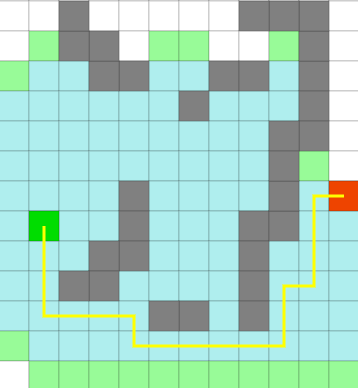
\includegraphics[width=0.3\linewidth]{./figures/grid-astar.png} \hspace{4pt}
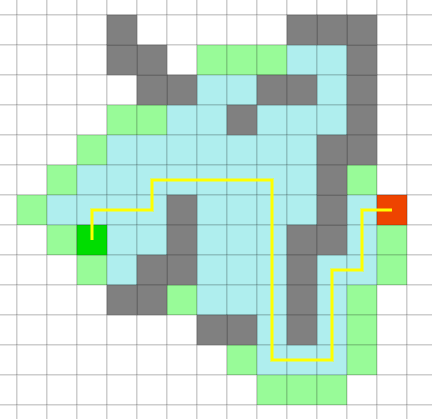
\includegraphics[width=0.3\linewidth]{./figures/grid-wastar-5.png} \hspace{4pt}
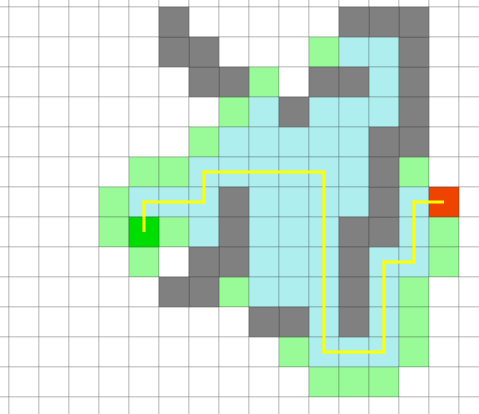
\includegraphics[width=0.3\linewidth]{./figures/grid-gbfs.png}
\caption{A*, wA*, GBFS比較}
\label{fig:grid-wastar}
\end{figure}

\subsection{貪欲最良優先探索 (Greedy Best-First Search)}
\label{sec:greedy-best-first-search}

wA*の例で見たように、$g$値に対して$h$値に重きを置くことによって解のクオリティを犠牲により高速に解を得ることができる。
問題によっては解のクオリティはあまり重要でなかったり、そもそもクオリティという概念がないことがある。
このようにとにかく解があればよいという場合は\define{貪欲最良優先探索}{Greedy Best-First Search}{どんよくさいりょうゆうせんたんさく}が使われることが多い \cite{wilt2010comparison}。

\begin{equation}
  f_{\text{gbfs}}(s) = h(s)
\end{equation}

貪欲最良優先探索は$g$値を無視し、$h$値のみで展開順を決定する。つまりwA*の$w$を無限大にしたものである。

貪欲最良優先探索は解のクオリティに保証がない。
しかし多くの問題で高速に解を発見できるとても強力な手法である。
図\ref{fig:grid-wastar}は貪欲最良優先探索である。wA*よりもさらに生成ノード数が少ないことが分かるだろう。



\section{上手く行かない場合}

ヒューリスティック探索が思ったより遅い場合考えるべきことはいくつかある。

まず考えるべきは、そもそもヒューリスティック探索によって解くべき問題なのかという点である。
制約プログラミングや他の組合せ最適化手法なら効率的な問題かもしれない。
似たような問題が他の手法によって解かれていないかを調べてみると良い。

ヒューリスティック探索が良さそうだと思ったら、試しにwA*にしてみて、weightを大きく取ってみよう。
おおまかに言うとwA*の実行速度はwの大きさに対して指数的に速くなる。w=1だと全く解けそうにない問題でもw=2にすると一瞬で解けることがある。
もしweightを10くらいにしてもすぐに解が発見できなければ、おそらくその問題で最適解を発見するのは非常に難しい。このような問題に対しては最適解を見つけることは諦め、局所探索 (\ref{ch:local-search}章)を使ったほうが良いだろう。
wA*でも解が見つけられない場合はそもそも解がない問題かもしれない。解がない場合は制約プログラミングのソルバーを使うと素早く検出できることが多い。

wA*で非最適解を見つけられる場合なら、工夫すればA*で最適解を見つけることができるかもしれない。
その場合まず、おおまかな探索空間の大きさを見積もり、そして1秒間に何ノードが展開されているかを確認すると良い。
ヒューリスティック探索の実行時間はおおまかには(展開するノード数)と(1ノードの展開にかかる時間)の積である。

%例えばA*探索はC++でスライディングタイル問題だと秒間XXXノードが展開できる。
もし秒間に展開されているノードの数が少ない場合、プロファイラを使ってどのオペレーションに時間がかかっているかを確認するべきだろう。多くの場合実行時間の大半をオープンリスト、クローズドリスト、ノードの展開関数(現在の状態とアクションから状態を計算する関数)のいずれかが占めている、ということがわかるだろう。

オープンリスト、クローズドリストの処理に時間がかかっている場合はデータ構造の改良によって問題が解決するかもしれない。効率的なデータ構造の設計については\ref{ch:search-performance}章を参照されたい。
あとはプロセスのメモリ消費量を確認してみよう。A*はメモリ消費も激しい。
実行時間が遅いのは、メモリを使いすぎていてメモリスワップが起きているからかもしれない。
より大きなメモリを使うか、IDA*などのメモリの消費量の少ない手法を試してみると良いかもしれない。

ノードの展開関数に時間がかかる場合はその実装を工夫するか、ノードの展開回数を最小限に抑えるしかない。
ノードの展開回数を減らす方法はなかなか難しいが、例えばヒューリスティック関数の改良によって可能である。
ほんの少しのヒューリスティック関数の改善によって探索の効率は劇的に上がりうる。
% 例えばスライディングタイル問題ではTODO。

これらの方法でもまだ解けない場合、扱っている問題は純粋なA*で解くには結構難しい問題かもしれない。
1968年にA*が初めて提案されてから、様々な発展手法が考案されてきた。
本書の後半で紹介する最新の手法を試してみれば解けるかもしれない。


\section{局所探索 (Local Search)}
\label{sec:local-search}

A*探索はクローズドリストに探索済みのノードを記憶しておくことでグラフ全体を見渡して探索を進める。しかし探索済みのノードをメモリにおいておくことは時間がかかるし、メモリも消費する。\define{局所探索}{local search}{きょくしょたんさく}は現在見つかった最良のノードのみを記憶しておくことで効率的に(最適とは限らない)解を発見する方法である。

\subsection{山登り法 (Hill Climbing)}
\label{sec:hill-climbing}
\define{山登り法}{hill climbing}{やまのぼりほう}は局所探索アルゴリズムであり、特に組み合わせ最適化問題のためのアルゴリズムとして使われる。
山登り法のアルゴリズムは非常に単純である。子ノードのうち最も$h$値が小さいノードを選ぶことを繰り返す。

\begin{algorithm}
\caption{山登り法 (Hill Climbing)}
	\Input{非明示的状態空間グラフ $(s, Goal, Expand, w)$, 評価関数 $h$}
	\Output{$s$からゴール状態$t \in T$への経路、経路が存在しなければ$\emptyset$}
	\While {$s \notin Goal$} {
	  $s' \leftarrow \arg \min_{s' \in Expand(s)} h(s)$\;
          $parent{s'} \leftarrow s$\;
          $s \leftarrow s'$\;
	}
	\Return $Path(s)$
\label{alg:hill-climbing}
\end{algorithm}

この手法は組み合わせ最適化・連続最適化のためによく使われる。
しかしグラフ探索アルゴリズムでこのまま使おうとすると評価関数の極小ではまってしまったり、デッドエンドに落ちてしまう可能性がある。


\subsection{強制山登り法 (Enforced Hill Climbing)}

ヒューリスティック探索でよく使われる局所探索は\define{強制山登り法}{enforced hill-climbing}{きょうせいやまのぼりほう} (EHC)である \cite{hoffmann2005ignoring}。
EHCは幅優先探索を繰り返し、現在のノードよりも$h$値が小さいノードを発見する。発見できればそのノードから再び幅優先を行い、ゴールを発見するまで続ける。もし$h$値が小さいノードが見つからなければ極小に陥ってしまったということであるので、探索を打ち切り、失敗 (Fail)を返す。

\begin{algorithm}
\caption{強制山登り法 (Enforced Hill Climbing)}
	\Input{非明示的状態空間グラフ $(s, Goal, Expand, w)$, 評価関数 $h$}
	\Output{$s$からゴール状態$t \in T$への経路、経路が存在しなければ$\emptyset$}
	\While {$s \notin Goal$} {
	  $T \leftarrow \{v \in Expand(s)\}$
	  $T' \leftarrow \{v \in T | h(v) < h(s) \}$
          \While {$T' = \emptyset$} {
            $T \leftarrow \{v \in Expand(u) | u \in T\}$
	    $T' \leftarrow \{v \in T | h(v) < h(s) \}$
          }
	  $s' \leftarrow \arg \min_{s' \in Expand(s)} h(s)$\;
          $parent{s'} \leftarrow s$\;
          $s \leftarrow s'$\;
	}
	\Return $Path(s)$
\label{alg:hill-climbing}
\end{algorithm}


ほとんどの局所探索アルゴリズムは完全性を満たさない。
なので解が発見できなければ(失敗を返す場合)続けてA*探索などを走らせないと解が発見できない場合がある。
山登り法などの局所探索の利点はなんといってもアルゴリズムはシンプルであり、実装が簡単であることである。
また、オープンリストなどのデータ構造を保持する必要がないので消費メモリ量が非常に少ない。

山登り法が記憶しなければならないノードは現在のノードとその子ノードらだけである。
毎回次のノードを選択したら、そのノード以外のノードは捨ててしまう。
貪欲最良優先探索(\ref{sec:greedy-best-first-search}節)も同様に$h$値のみしか見ていないが、すべての生成済みノードをオープンリストに保存して評価値を確認していることと比較すると、山登り法がいかにアグレッシブな手法であるかがうかがえるだろう。



\section{関連文献}

\define{最良優先探索}{best-first search}{さいりょうゆうせんたんさく}は2種類の定義があることに注意したい。
本書では最良優先探索をA*を含む、何らかの有望さの指標に従ってグラフを探索するアルゴリズムの集合を指す。
一方、ゴールに最も近いと考えられるノードを常に最優先して展開するアルゴリズムを特に最良優先探索と呼ぶことも多い。本書ではこの方法は貪欲最良優先探索と呼んでいる。

同じ問題に対して重み付きA*を繰り返し$w$値をだんだんと小さくしていくことでだんだんと解のクオリティを向上させることができる。
この方法をAnytime A*と呼ぶ \cite{likhachev2004ara} \footnote{一般にいつ停止しても現時点で見つかった中で一番良い(最適とは限らない)解を返し、時間をかけるほど解のクオリティを改善していくアルゴリズムをanytimeアルゴリズムと呼ぶ。}。

本書で扱わない重要な探索アルゴリズムとして遺伝的アルゴリズムがある \cite{goldberg1989}。
遺伝的アルゴリズムはさまざまな最適化問題に適用できる。
グラフ探索問題で使われることは少ないが、グラフ探索問題ではなかなか解けない難しい問題が遺伝的アルゴリズムによって簡単に解けることがある。例えばN-Queen問題はチェスの盤面上にクイーンを互いに移動可能範囲がぶつからないように配置する問題であるが、これはグラフ探索の手法だとなかなか解くのが難しいが遺伝的アルゴリズムだと非常に効率的に解けることが知られている。
